\cotefile{156-8}
\scanpage{98}\mspage{89}
\uline{2 juillet}\qquad Déterminons maintenant les \uline{figures}. Tout drapeau $T$ \deleted{(\unsure{non} vide) de $L$} détermine une figure\deleted{\unsure{,|.}} $F_T$, savoir \deleted{\unsure{celle} \unsure{formée|que} \unsure{l'en}} 
\[
 F_T=\{X\in\unsure{M|\mathcal M}\mid X\ \text{\unsure{interstitiel|intersticiel} pour }T\},
\]
qu'on se représente graphiquement par
\figure{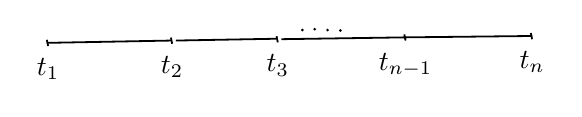
\begin{tikzpicture}[x=.78cm,y=.58cm,line width=.65pt]
\draw (0,0)--(2.0,.05) (2.08,.05)--(3.72,.09) (3.8,.08)--(5.82,.12)--(7.88,.15);
\foreach \x/\y/\lab in {0/0/{t_1},2.02/.05/{t_2},3.74/.08/{t_3},5.82/.12/{t_{n-1}},7.88/.15/{t_n}}{
 \draw (\x,\y-.07)--(\x-.02,\y+.065);
 \node[below=2pt] at (\x,\y) {$\lab$};}
\foreach \x/\y in {4.14/.28,4.34/.30,4.55/.28,4.76/.27}{\fill (\x,\y) circle (.53pt);}
\end{tikzpicture}}
(en ``oubliant'' les éléments de $L$ qui ne sont pas dans un des segments $[t_i,t_{i+1}]$, $1\leq i\leq n-1$. Les cas ``dégénérés'' sont \deleted{$T=\varnothing,\ F_{\varnothing}=\varnothing$}
% slanted
\margin{\uline{NB} $F_T$ détermine $T$ \unsure{par} $T=\delta F_T$}
\[
\begin{aligned}
 T=\varnothing &\Rightarrow F_T=\varnothing &&\text{graphisme :} && ?\\
 T=\{\deleted{\unsure{t}}\unsure{a|t}\} &\unsure{\Rightarrow|\mathrel{=}} F_T=\{P_{\deleted{\unsure{t}}\unsure{a|t}}\} &&\text{graphisme :} &&
 \vcenter{\hbox{\begin{minipage}{1.65cm}\figure{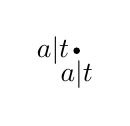
\begin{tikzpicture}[baseline]
 \node at (-.30,0) {$\deleted{\unsure{a|t}}$};
 \fill (0,0) circle (1.2pt) node[below] {$\unsure{a|t}$};
 \end{tikzpicture}}\end{minipage}}}\\
 T=\{\unsure{a|t},b\} &\Rightarrow F_T=\widetilde{S_{\unsure{a|t},\unsure{b|t_2}}} &&\text{graphisme} &&
 \vcenter{\hbox{\begin{minipage}{1.65cm}\figure{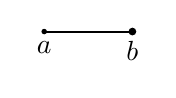
\begin{tikzpicture}
 \draw[line width=.7pt] (0,0) node[below] {$a$}--(1.12,0) node[below] {$b$};
 \fill (0,0) circle (1pt) (1.12,0) circle (1.4pt);
 \end{tikzpicture}}\end{minipage}}}
\end{aligned}
\]
après ça, on a
\figure{\begin{tikzpicture}[x=1cm,y=.65cm,line width=.65pt]
\draw[fill=white] (0,0) circle (1.3pt);
\draw (.075,0)--(1.55,.035) (1.64,.025)--(2.94,.035);
\draw[fill=white] (2.96,.035) circle (1.3pt);
\fill (1.54,.03) circle (1.2pt);
\node[below] at (0,0) {$a$};\node[below] at (1.55,0) {$b$};\node[below] at (3,0) {$c$};
\node at (7,.1) {etc.};
\end{tikzpicture}}

Sur l'ens des drapeaux \uline{non vides} $\mathrm{Drap}^{\unsure{*|\times}}(L)$ on met une relation d'ordre
\[
 T<T'\quad\text{\unsure{sss}}\quad \forall\,t\in T,t'\in T',\ \text{on a }t<t',
\]
% slanted
\margin{NB $T<T'$ (ou encore $T\parallel T'$ dans l'ens ordonné $\mathrm{Drap}^{*}(L)$) implique $T\cap T'=\deleted{\unsure{e}}\varnothing,\ T\cup T'\in\mathrm{Drap}^{*}(L)$}
qui nous permet de considérer des drapeaux de drapeaux.

\uline{Lemme} Soient $T,T'\in\mathrm{Drap}^{*}(L)$, pour que $F_T\parallel F_{T'}$ ($\Leftrightarrow F_T\mathrel{|\circ|}F_{T'}$) il \unsure{f. et s.} que $T\parallel T'$ \inserted{dans $\mathrm{Drap}^{*}(L)$} i.e. $\{T,T'\}\in\mathrm{Drap}^{*}(\mathrm{Drap}^{*}(L))$.
% archive sheet number: 98
